\documentclass[a4paper,12pt,oneside,English]{article}
\usepackage[a4paper,top=1.5cm,bottom=1.5cm,left=1cm,right=1cm]{geometry}
\usepackage[utf8]{inputenc}
\usepackage[T1]{fontenc}
\usepackage{blindtext}
\usepackage{framed}
\usepackage[svgnames]{xcolor}
\usepackage{graphicx}
\definecolor{shadecolor}{gray}{0.9}
\usepackage{mathtools}
\usepackage{caption}
\usepackage{subcaption}
\usepackage{dsfont}
\usepackage{nccmath}
\usepackage{graphicx}
\usepackage{amsthm}
\usepackage{color} 
\usepackage[pdftex,backref,linktocpage,colorlinks]{hyperref}
\usepackage{xcolor}
\usepackage{empheq}
\usepackage{adjustbox}
\usepackage{graphicx}
\usepackage{amssymb}
\usepackage{amsmath}
\usepackage{siunitx}
\usepackage{framed}
\usepackage{graphicx}
\documentclass[xcolor=table]{beamer}
\usepackage[table,xcdraw]{xcolor}
\usepackage[authoryear]{natbib}
\hypersetup{
    colorlinks,
    linkcolor={red!50!black},
    citecolor={red!50!black},
    urlcolor={red!50!black}
}
\usepackage{titling}
\usepackage{fancyhdr}
\usepackage[shortlabels]{enumitem}
\usepackage{float}
\usepackage[nottoc, notlof]{tocbibind}
\usepackage{setspace}
\usepackage[T1]{fontenc}
\usepackage{amsfonts}
\usepackage{amsmath}
\usepackage{indentfirst}
\renewcommand{\baselinestretch}{1.5}
\setlength{\skip\footins}{5ex plus 4pt minus 2pt}
\usepackage{rotating}
\usepackage{tocloft}
\setlength{\cftaftertoctitleskip}{1cm}
\setlength{\cftafterloftitleskip}{1cm}
\usepackage{enumitem}
\usepackage{titletoc,tocloft}
\setlength{\cftsubsecindent}{0cm}
\usepackage{floatflt} 
 \usepackage[bf, small]{caption}
 \usepackage[justification=centering]{caption}
 \setcounter{secnumdepth}{0}
\title{Problem Set 2 - Econometrics}
\author{ Giacomo Lo Conte, Kun Wu, Francesca Eustacchi, Neeharika Kakunuri, Noor Ahmed Khoso }

\begin{document}

\maketitle
\section{1. Theory}
\textbf{a. Consider a case where $Z$ is a binary instrument, $T$ is a discrete multi-valued treatment $(T_Z \in {0,1,2,...,J})$, $T = Z T_1 + (1 - Z)T_0$ is the observed level of treatment, and $Y$ is the outcome. Assume that the random variables $T_0, T_1, Y_0, Y_1, . . . , Y_J$ are jointly independent of $J$ and that the level of treatment is higher when $Z = 1$ than when $Z = 0$, i.e. $T_1 - T_0 \geq 0$. Further, assume that $Pr(T_1 \geq j \geq T_0) > 0$ for at least one $j \in {0,1,2,...J}$, which means that the instrument on average affects the level of treatment. Show that under these assumptions the Wald estimator is a weighted average of the causal response of a unit change in treatment,}
\begin{equation}
    \cfrac{E[Y| Z = 1] - E[Y | Z = 0]}{E[T| Z = 1] - E[T| Z = 0]} = \sum^J_{j=1} \omega_j  E[Y_{j1} - Y_{j0}|T_1 \geq j > T_0],
\end{equation}
\textbf{where the weight are }
\begin{equation}
\omega_j = \cfrac{Pr(T_1\geq j > T_0)}{\sum^J_{i=1}Pr(T_1\geq i > T_0)}
\end{equation}

Consider separately the numerator and the denominator of the Wald Estimator. We will start proving that the latter is equal to $\sum_{j=1}^J Pr(T_1\geq j>T_0)$.

First of all consider what $E[T|Z=1]$ represents. Since $T$ is a multi-valued discrete treatment, it represent the average value $\bar T$ of the treatment, conditioned on the share of the population who received Z. So it can be written as the weighted average of the various $E[T=T_j|Z=1]$ using the share of population receiving $T_j$ ($\pi_j$) as the weights.

\[
E[T|Z=1]=\sum_{j=1}^J E[T=T_j|Z=1] \pi_j
\]

By the LATE Theorem we can decompose further $E[T=T_j|Z=1]$. By the assumptions that $T_1>T_0$ and $Pr(T_1 \geq j \geq T_0) > 0$ we can argue that the instrument fulfills monotonicity and there are no defiers. Moreover, since the instrument is as good as random, this means that distributed in the population independently on the distribution of $\pi_j$. We can write this as $E[\pi_A|\pi_j]=\pi_A,E[\pi_N|\pi_j]=\pi_N,E[\pi_C|\pi_j]=\pi_C,\forall j$, where $\pi_A, \pi_N$ and $\pi_C$ are respectively the shares of the population of always-takers, never-takers and compliers. In mathematical terms, we can write that as:

\[
\begin{split}
E[T=T_j|Z=1]&=E[T=T_j|Z=1, always-takers]\pi_A+\\&+E[T=T_j|Z=1, never-takers]\pi_N+\\&+E[T=T_j|Z=1, compliers]\pi_C
\end{split}
\]

Notice that for $j\in\{0,J\}$ we would witness two extreme cases. Indeed, by definition $E[T=T_0|Z=1, compliers]=E[T=T_0|Z=1, always-takers]=E[T=T_J|Z=1, never-takers]=0$. If this were not true, then the units exhibiting such behaviours would not be considered in those groups.

Now consider the second term $E[T|Z=0]$. We can reason at the same way and split the term in the weighted sum of all different $E[T=T_j|Z=0]$. Again, we can apply again the LATE theorem and decompose additionally. From the randomness of the instrument assumption, we know that $E[T_j|Z=1, k]=E[T_j|Z=0, k]$ for $k\in\{ALW,NEV\}$. The difference, then, is:
\[
E[T=T_j|Z=1]-E[T=T_j|Z=0]=E[T=T_j|Z=1, COM]\pi_C-E[T=T_j|Z=0, COM]\pi_C
\]

Since this is not a discrete multi-valued case, we need to spend some time to interpret what this represents. The LATE in this case is even more "local" then the binary case. Indeed, it represents the difference between those compliers who receive $T_j$ because treated by $Z$ and those who are not treated, otherwise they would have received $T_{j+1}$. In other words, they belong to two different groups of the population. To have comparable groups we need to observe the difference between $E[T=T_j|Z=1, COM]$ and $E[T=T_{j-1}|Z=0, COM]$. This is possible when we take the sum of that:
\[
E[T|Z=1]-E[T|Z=0]=\sum_{j=1}^J \pi_j \pi_C(E[T_j|Z=1, COM]-E[T_{j-1}|Z=0, COM])
\]

This term can be seen as the product of two probabilities:
\begin{itemize}
    \item $\pi_j^*\pi_C$: the share of compliers in the subpopulation that receive $T_j$;
    \item $E[T_j|Z=1, COM]-E[T_{j-1}|Z=0, COM]$: the marginal effect on $T_j$ of the instrument $Z$.
\end{itemize}

Since they are independent, their product represent the joint probability of being a unity in $j$, receiveing $Z$ and increasing from $T_0$ to $T_1$. In math:
1[]
E[T|Z=1]-E[T|Z=0]=\sum_{j=1}^J Pr(T_1\geq j>T_0) 
\]

For the numerator the reasoning is very similar. First we decompose $E[Y|Z=1]$ and $E[Y|Z=0]$ as a weighted average of the population groups. Then we can decompose further $E[Y=Y_j|Z=1]$ and $E[Y=Y_j|Z=0]$ using the LATE theorem. Recalling that $E[Y=Y_j|Z=1, ALW]=E[Y=Y_j|Z=0, ALW]$ and $E[Y=Y_j|Z=1, NEV]=E[Y=Y_j|Z=0, NEV]$, the LATE of $Y_j$ is:
\[
E[Y=Y_j|Z=1]-E[Y=Y_j|Z=0]=(E[Y=Y_j|Z=1, COM]-E[Y=Y_j|Z=0, COM])\pi_C
\]

However, again, the two terms refers to two different subgroups of the population, then by taking the sum in $j$, we can define:
\[
E[Y|Z=1]-E[Y|Z=0]=\pi_C\sum_{j=1}^J E[Y_{j1}-Y_{j0}|COM, Z] Pr(T_1\geq j T_0)
\]

Notice that 

\textbf{b) Provide an interpretation of both factors on the RHS if Equation (1), i.e . $E [Y_j − Y_j−1 | T1 \geq j > T_0]$
and $\omega_j$. What does the presence of both factors teach us about the local average treatment effect?\\
c) In the lecture we have proven that in absence of defiers the IV estimate for an outcome $Y_i$, a binary treatment $D_i$ and a binary instrument $Z_i$ is
\begin{equation}
    \beta^{IV*} = E(Y_i|D_i = 1) - E(Y_i|D_i = 0)) = E(Y_i_1 - Y_i_0|complier)
\end{equation}
Now suppose the share of defiers is $0 < \pi_D < 1$.}
\begin{enumerate}[i)]
    \item \textbf{Derive the IV estimate for this case.}
    \item \textbf{Assume that $\pi_D = a × \pi_C$ with $0 < a < 1$ and $\beta^{IV*}> 0$. Discuss whether additional, plausible assumptions on $E(Y_i_1 - Y_i_0|defier)$ allow you to recover a lower bound for $\beta^{IV*}$.}
\end{enumerate}

The Wald Estimator formula is:
\[
\hat\beta^{IV}=\cfrac{E[Y|Z=1]-E[Y|Z=0]}{E[D|Z=1]-E[D|Z=0]}
\]

Focus on the numerator. Let consider the first term $E[Y|Z=1]$. Recalling that Z is as good as random, we can state the distribution of always-takers, never-takers, compliers and defiers is expected to be the same as in the population. Call these values respectively as $\pi_A,\,\pi_N,\,\pi_C,\,\pi_D$. The term, thus, can be decomposed as:

\[
\begin{split}
    E[Y|Z=1]=&E[Y|Z=1, always-takers]\pi_A+E[Y|Z=1, never-takers]\pi_N+\\
    +&E[Y|Z=1, compliers]\pi_C+E[Y|Z=1, defiers]\pi_N
\end{split}
\]

Conversely, the second term $E[Y|Z=0]$ is:

\[
\begin{split}
    E[Y|Z=0]=&E[Y|Z=0, always-takers]\pi_A+E[Y|Z=0, never-takers]\pi_N+\\
    +&E[Y|Z=0, compliers]\pi_C+E[Y|Z=0, defiers]\pi_N
\end{split}
\]

The difference between the two terms represent the effect of the instrument on the outcome. The instrument, though, impacts on the outcome only through the treatment variable D. For this reason, both for always-takers and never-takers this difference is not significant. Indeed, both groups will be exposed (or not) to the treatment regardless the value of Z, i.e. $E[Y|Z=1,always-takers]=E[Y|Z=0,always-takers]$ and $E[Y|Z=1,never-takers]=E[Y|Z=0,never-takers]$. The numerator, hence, can be written as:

\[
\begin{split}
E[Y|Z=1]-E[Y|Z=0]&=E[Y|Z=1,compliers]-E[Y|Z=0,compliers])\pi_C+\\&+(E[Y|Z=1,defiers]-E[Y|Z=0,defiers])\pi_D
\end{split}
\]

Focus now on the denominator. Notice that $E[D|Z=1]$ represents the share of units that receive the treatment (D=1) having received the instrument (Z=1). This population is composed only by always-takers and compliers, however we cannot distinguish who is whom. However, since the instrument is as good as random, we can state that the distribution of always-takers and compliers in this group is expected to be the same as the distribution in the population. In other words $E[D|Z=1]=\pi_A-\pi_C$. Now observe $E[D|Z=0]$. It represents the share of units that receive the treatment (D=1) without having received the instrument (Z=0). This population is composed by always-takers and defiers. For the same reason as before, $E[D|Z=0]=\pi_A-\pi_D$. The denominator hence can be rewritten as $E[D|Z=1]-E[D|Z=0]=\pi_C-\pi_N$.

The Wald Estimator, therefore, can be written as:

\[
\hat\beta^{IV*}=\cfrac{(E[Y|Z=1,Com]-E[Y|Z=0,Com])\pi_C+(E[Y|Z=1,Def]-E[Y|Z=0,Def])\pi_D}{\pi_C-\pi_N}
\]

Assuming that $\pi_D=a\pi_C$:

\[
\hat\beta^{IV*}=\cfrac{E[Y|Z=1,Com]-E[Y|Z=0,Com]+(E[Y|Z=1,Def]-E[Y|Z=0,Def])a}{1-a}
\]

Since the true parameter is represented by the effects on the compliers:
\[
E[\hat\beta^{IV*}]=\cfrac{\beta}{1-a}+\cfrac{a}{1-a}(E[Y|Z=1,Def]-E[Y|Z=0,Def])
\]

To have a lower bound we have to assume that the bias we observe is negative. In other words we need $E[Y|Z=1,Def]<E[Y|Z=0,Def]$. From definition of defiers, we can write $E[Y|Z=1, Def]=E[Y_{i0}|Def]$ and $E[Y|Z=0, Def]=E[Y_{i1}|Def]$, then we need to assume $E[Y_{i0}|Def]<E[Y_{i1}|Def]$. We think this is a reasonable assumption to make, since it implies that the effect of the treatment on defiers follows the same direction it does in the rest of the population. However, for very small values of \textit{a} the value of the bias is negligible.



\newpage


\section{2. Simulation Exercise}

\textbf{An important property of the IV estimator is that it is biased in small samples but consistent. For this reason one should never write that an IV estimator is used to obtain unbiased estimates. We want to better understand the small sample properties through simulations of the sampling distribution of IV and OLS estimators. In all simulations, let x, y, z, u and ε be random variables and assume the data-generating process:}

\begin{equation}
    y = \alpha+\beta x+ \epsilon
\end{equation}

\begin{equation}
    x = \gamma_0+\gamma_1z+ u
\end{equation}

\textbf{Set the parameter $\beta = 1$ and, unless required otherwise, $\alpha = \gamma_0 = 0$. Moreover, construct $\epsilon$ such that it's Pearson correlation with \textit{x} is 0.4.}


\subsection{a) Sampling Distribution under strong instruments}

\textbf{Construct the instrument $z$ such that its Pearson correlation with \textit{x} is 0.5 while its correlation with $\epsilon$ is zero. Consider four different sample sizes: $N = 50$, $N = 100$, $N = 250$ and $N = 1000$. For each sample size, run at least 10,000 simulations whereby you estimate $\beta^{OLS}$ and $\beta^{IV}$ (choose fewer replications if you have problems with computing power). In the same graph, plot the sampling distributions for OLS and IV for all four sample sizes. Discuss the difference in shape of the sampling distributions between OLS and IV.}

We constructed $x$, $z$ and $\epsilon$ through a random extraction of 10,000 observations. The three variable are correlated as required. Notice that, once we defined these three, the value of $\gamma_1$ can be defined as $\rho_{xz}\cfrac{\sigma_x}{\sigma_z}$. Its value then is defined by the ratio of the standard deviations, that are$\sigma_x=\sigma_z=\sigma_\epsilon=1$. In the second step, we derive $y=x+\epsilon$.

Among our population of 10,000 of units, we run a bootstrap (10,000 iterations) of our OLS and IV estimates over four different samples.
Graphics in figure \ref{Cor50} show clearly how the distributions of the the IV and OLS estimates change when the sample size increases.

\begin{figure}[p!]
    \begin{minipage}[b]{0.5\linewidth}
        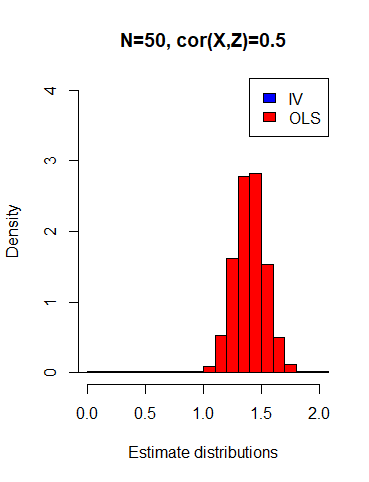
\includegraphics[width=\linewidth]{Fig1.png}
    \end{minipage}
    \begin{minipage}[b]{0.5\linewidth}
        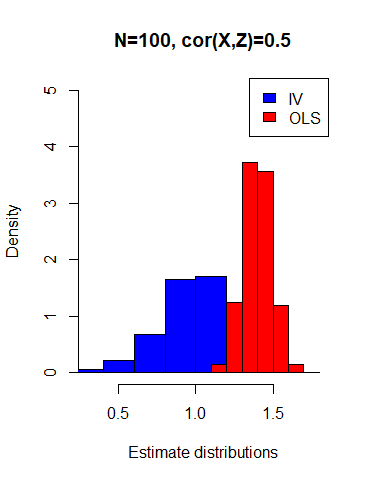
\includegraphics[width=\linewidth]{Fig2.png}
    \end{minipage}
    \begin{minipage}[b]{0.5\linewidth}
        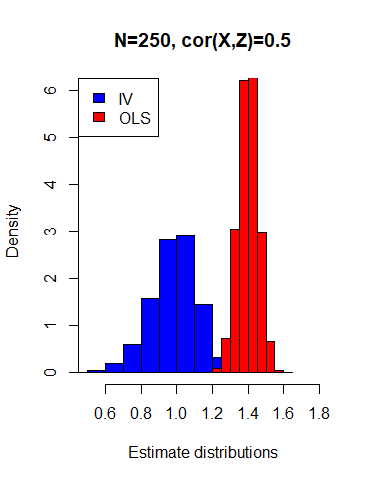
\includegraphics[width=\linewidth]{Fig3.png}
    \end{minipage}
    \begin{minipage}[b]{0.5\linewidth}
        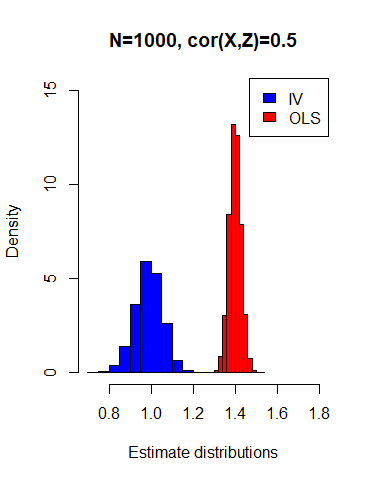
\includegraphics[width=\linewidth]{Fig4.png}
    \end{minipage}\hfill
    \label{Cor50}
    \caption{Distributions of IV and OLS estimates when $\rho_{XZ}=0.5$}
\end{figure}

How we can see, as long as the sample size increases we see that the distribution variance decreases both for the OLS and IV estimator. This is the graphic representation of the consistency property. Moreover, we can see graphically also the demonstration of the efficiency property of the OLS. OLS indeed shows a consistent lower variance and the frequency of the median values rises faster. In other words, IV estimator distribution is flatter than the OLS one. However, it is evident that OLS distribution biased, contrary to the IV. Indeed, while the IV estimator distribution is centered on 1, the OLS distribution is centered around 1.4. The bias is positive and is exactly equal to $\cfrac{Cov(x,\epsilon)}{\sigma^2_x}$. Since $Cov(x,\epsilon)=\rho_{x\epsilon}\sigma_x$, the bias is equal to $\cfrac{\rho_{x\epsilon}}{\sigma_x}\approx 0.4$. From these graphs, then it is clear that, in a non-biased setting the IV estimates may have more problems with the statistical inference. The IV errors are indeed larger than the OLS.

\subsection{b) Weaker instruments:}
\textbf{Now repeat the analysis from a), but instead assume that the correlation between the instrument $z$ and the regressor $x$ is $0.15$. Discuss the difference in sampling distributions between OLS and IV and, in addition, discuss the difference between sampling distributions based on weak and strong IVs.}

\begin{figure}[p!]
    \begin{minipage}[b]{0.5\linewidth}
        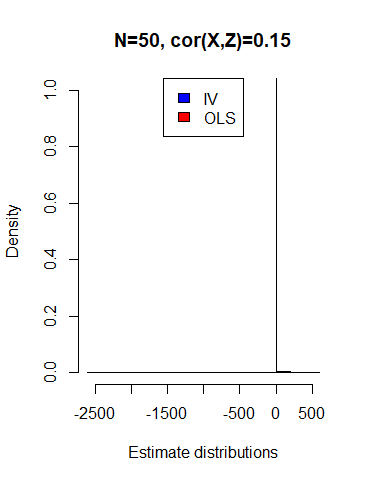
\includegraphics[width=\linewidth]{Fig1A.png}
    \end{minipage}
    \begin{minipage}[b]{0.5\linewidth}
        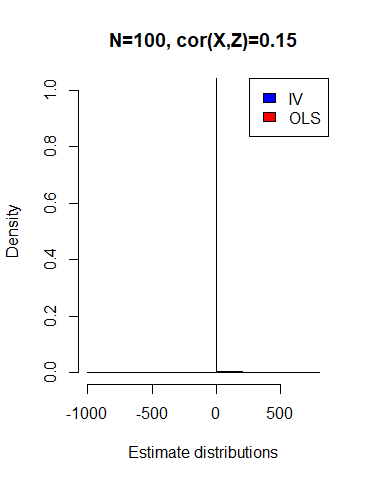
\includegraphics[width=\linewidth]{Fig2A.png}
    \end{minipage}
    \begin{minipage}[b]{0.5\linewidth}
        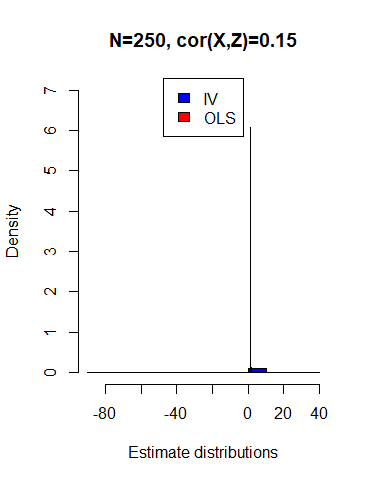
\includegraphics[width=\linewidth]{Fig3A.png}
    \end{minipage}
    \begin{minipage}[b]{0.5\linewidth}
        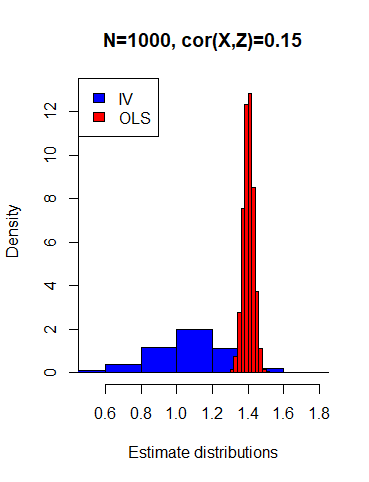
\includegraphics[width=\linewidth]{Fig4A.png}
    \end{minipage}\hfill
    \label{cor15}
    \caption{Distributions of IV and OLS estimates when $\rho_{XZ}=0.15$}
\end{figure}

In figure \ref{cor15} we can hardly observe the OLS distribution for a problem of scale, however it remains basically unchanged. In the IV case, we can notice a very different scenario. The IV distribution is much flatter than the previous case. To fully grasp the difference we can observe the scale of the axes. While in figure \ref{Cor50}, the top-right graph presents an interval between 0.3 and 1.7, in figure \ref{cor15} the same graph the interval is between -1000 and 600. This is due to the formula of the variance for the IV estimator. The asymptotic variance of the IV is:
\[
\widehat{Avar}(\beta^{IV}-\beta|X,Z)=E[(Z'X)^{-1}Z'uu'Z(Z'X)^{-1}|X,Z]
\]
\[
\widehat{Avar}(\beta^{IV}-\beta)=E[uu'](Z'X)^{-1}=\Sigma^2_u(Z'X)^{-1}
\]
The asymptotic variance of the IV estimator can be written as the variance matrix of the error times the inverse of the covariance of Z and X. In our simple univariate case $Z'X=Cov(x,z)=\rho_{xz}\sigma_z\sigma_x$=. The variance of the estimator, then, is inversely related to $\rho_{xz}$. For this reason, the weaker is the instrument and the higher is the variance of the IV estimator. This leads to problems for the statistical inference since the results are not significant even if unbiased.

\newpage
\section{Empirical Application}

The empirical application is based on a cross-sectional dataset assign2.dta, which contains the following variables:
\begin{itemize}
    \item \textit{age}: age of surveyed individual
    \item \textit{logearn}: log annual earnings
    \item \textit{yob}: year of birth
    \item \textit{schooling}: age at which the person left school.
\end{itemize}
a) The goal is to estimate the returns to education. For this purpose, estimate an OLS regression of \textit{logearn} on schooling, controlling for fourth-order polynomials in age and year of birth. Interpret the coeffcient of schooling.\\


\begin{table}[!htbp] \centering 
  \caption{Regression Summary: OLS with controlling for 4th order polynomial for age and yob} 
  \label{reg 1} 
\begin{tabular}{@{\extracolsep{5pt}}lc} 
\\[-1.8ex]\hline 
\hline \\[-1.8ex] 
 & \multicolumn{1}{c}{\textit{Dependent variable:}} \\ 
\cline{2-2} 
\\[-1.8ex] & logearn \\ 
\hline \\[-1.8ex] 
 schooling & 0.158$^{***}$ \\ 
  & (0.002) \\ 
  & \\ 
 age & $-$0.254 \\ 
  & (0.540) \\ 
  & \\ 
 age\_sq & 0.009 \\ 
  & (0.017) \\ 
  & \\ 
 age\_cube & $-$0.0001 \\ 
  & (0.0002) \\ 
  & \\ 
 age\_4 & 0.00000 \\ 
  & (0.00000) \\ 
  & \\ 
 yob & 0.441$^{*}$ \\ 
  & (0.252) \\ 
  & \\ 
 yob\_sq & $-$0.018 \\ 
  & (0.012) \\ 
  & \\ 
 yob\_cube & 0.0003 \\ 
  & (0.0002) \\ 
  & \\ 
 yob\_4 & $-$0.00000 \\ 
  & (0.00000) \\ 
  & \\ 
 Constant & 1.489 \\ 
  & (6.176) \\ 
  & \\ 
\hline \\[-1.8ex] 
Observations & 30,801 \\ 
R$^{2}$ & 0.147 \\ 
Adjusted R$^{2}$ & 0.147 \\ 
Residual Std. Error & 0.494 (df = 30791) \\ 
F Statistic & 591.542$^{***}$ (df = 9; 30791) \\ 
\hline 
\hline \\[-1.8ex] 
\textit{Note:}  & \multicolumn{1}{r}{$^{*}$p$<$0.1; $^{**}$p$<$0.05; $^{***}$p$<$0.01} \\ Values in the parentheses are the standard errors.\\The dependent variable is logged earnings.
\end{tabular} 
\end{table}
In table \ref{reg 1} , we present the regression summary of the simple OLS model while controlling for the fourth order polynomials of age and year of birth. In the table, we see that the estimate for schooling is significant at 1\%. Where as the estimate for year of birth is also significant at 10\%. We see that with an additional year of schooling there is 15.8 \% increase in earnings. This is only true when we control for higher order polynomials in our regression. In order for us to not to over-fit or under-fit the model we use the higher order polynomial. Additionally, despite adding the higher order polynomials we see the estimated $R^2$ and the $Adjusted R^2$  is 14.7\%\\

An additionally step carried out is to compare the model from table \ref{reg 1} to table \ref{reg 2}. As we can see the results in the table \ref{reg 2}
are the summary findings when we do not have higher order polynomials. We simply estimate the logged earnings as a function of age , year of birth (yob) and schooling. In this particular regression, we see that all the variables are significant at 90\%. Additionally, the estimate for schooling is 15.7 indicating that there is rise in earnings by 15.7\% with an additional year of schooling. This estimate in particular very close to the estimate obtained in table \ref{reg 1}. The adjusted$R^2$ and the $R^2$ in this case is comparatively smaller at 14\%. Therefore, we can conclude by saying that using the higher order polynomials is a better fit.\\
is A common way to obtain causal estimates is to use changes in compulsory schooling laws for identification. In this case, birth cohorts born before 1933 $(yob<33)$ had to go to school until they were 14 years old, whereas compulsory schooling age was raised to 15 years for all cohorts born from 1933 onwards. This change in compulsory schooling laws can be used as an instrumental variable for the actual duration of schooling. The instrument is a dummy LAW that equals unity if a person is born 1933 or later and zero otherwise.
\begin{table}[!htbp] \centering 
  \caption{Regression Summary: A Simple OLS Model} 
  \label{reg 2} 
\begin{tabular}{@{\extracolsep{5pt}}lc} 
\\[-1.8ex]\hline 
\hline \\[-1.8ex] 
 & \multicolumn{1}{c}{\textit{Dependent variable:}} \\ 
\cline{2-2} 
\\[-1.8ex] & logearn \\ 
\hline \\[-1.8ex] 
 age & 0.005$^{***}$ \\ 
  & (0.001) \\ 
  & \\ 
 yob & 0.005$^{***}$ \\ 
  & (0.001) \\ 
  & \\ 
 schooling & 0.157$^{***}$ \\ 
  & (0.002) \\ 
  & \\ 
 Constant & 2.964$^{***}$ \\ 
  & (0.055) \\ 
  & \\ 
\hline \\[-1.8ex] 
Observations & 30,801 \\ 
R$^{2}$ & 0.140 \\ 
Adjusted R$^{2}$ & 0.140 \\ 
Residual Std. Error & 0.496 (df = 30797) \\ 
F Statistic & 1,673.896$^{***}$ (df = 3; 30797) \\ 
\hline 
\hline \\[-1.8ex] 
\textit{Note:}  & \multicolumn{1}{r}{$^{*}$p$<$0.1; $^{**}$p$<$0.05; $^{***}$p$<$0.01} \\ The vales in the parentheses are standard errors\\(This regression is additional & used to compare regression with 4th order polynomial)
\end{tabular} 
\end{table} 
\textbf{b) Discuss this instrument in theory, assuming that schooling Si is related to the instrument $Z_i$ by the latent assignment mechanism
\begin{equation*}
    S_i = 1(\gamma_0+ \gamma_1 Z_i > \eta_i),\;\; with\;\; E(Z_i \eta _i) = 0
\end{equation*}
The random variable $\eta_i$ represents the individual resistance to treatment. Why could there be a
first stage? Under what condition is this instrument valid? What are potential threats to validity?
Furthermore, explain who are the compliers, always-takers and never-takers in this case. Would the IV estimate correspond to the average treatment effect (why or why not)?}\\
\textbf{c) As in any good empirical project, begin with a graphical inspection of the relationships of interest. This is best done through binscatters. Produce and discuss the graphs listed below. In all graphs, include a vertical line at $yob=33$.
\begin{itemize}
    \item Plot the probability that a person leaves school before age 15 against the year of birth.
    \item Binscatter of schooling and year of birth
    \item Binscatter of log earnings and year of birth.
\end{itemize}}
\textbf{d) Calculate the Wald estimator (without controls) "by hand", i.e. based on conditional averages. Compare your results to those of a 2SLS estimation based on an inbuilt command (e.g. \textit{ivregress} in Stata or \textit{ivreg} in R). Interpret your results and compare them to the OLS results in a).}\\

In table \ref{reg 3}, we present the summary of findings fro the regression of Outcome  \textit(logearn) and instrument variable \textit(LAW). We see that the instrument i.e, the LAW or compulsory schooling up to age 15 years rises the probability of schooling for an additional year by 99 units. The estimate for the instrument is statistically significant  at 10\%. The adjusted $R^2$ 13.6\% also explains the moderate yet significant impact of the instrument, which is definitely an incentive. We will discuss the impact it has on earnings. And this is the first stage regression in IV estimation.
We can, in simple words say that the law of compulsory schooling of 15 years is a valid instrument,  gain of an additional year of schooling has an indirect impact on earnings via schooling. We will present a formal discuss of this proposition below.\\
\begin{table}[!htbp] \centering 
  \caption{Regression Summary : Treatment and Instrument} 
  \label{reg 3} 
\begin{tabular}{@{\extracolsep{5pt}}lc} 
\\[-1.8ex]\hline 
\hline \\[-1.8ex] 
 & \multicolumn{1}{c}{\textit{Dependent variable:}} \\ 
\cline{2-2} 
\\[-1.8ex] & schooling \\ 
\hline \\[-1.8ex] 
 LAW & 0.990$^{***}$ \\ 
  & (0.014) \\ 
  & \\ 
 Constant & 14.624$^{***}$ \\ 
  & (0.012) \\ 
  & \\ 
\hline \\[-1.8ex] 
Observations & 30,801 \\ 
R$^{2}$ & 0.137 \\ 
Adjusted R$^{2}$ & 0.136 \\ 
Residual Std. Error & 1.146 (df = 30799) \\ 
F Statistic & 4,868.939$^{***}$ (df = 1; 30799) \\ 
\hline 
\hline \\[-1.8ex] 
\textit{Note:}  & \multicolumn{1}{r}{$^{*}$p$<$0.1; $^{**}$p$<$0.05; $^{***}$p$<$0.01} \\ The values in parenthesis are standard errors.
\end{tabular} 
\end{table} 
In table \ref{reg 4} we present a formal discussion of the results of imposing the law of compulsory schooling up-to 15 years and returns to education. As we can see, the estimate obtained is 0.162, indicating that upon the imposition of the law, earnings are likely to increase by 16.2\% provided an individual complies with the law. And this casual inference occurs via schooling which in our case is the treatment. We call this the reduced form or intention to treat (ITT).
\begin{table}[!htbp] \centering 
  \caption{Regression Summary: Outcome and Instrument} 
  \label{reg 4} 
\begin{tabular}{@{\extracolsep{5pt}}lc} 
\\[-1.8ex]\hline 
\hline \\[-1.8ex] 
 & \multicolumn{1}{c}{\textit{Dependent variable:}} \\ 
\cline{2-2} 
\\[-1.8ex] & logearn \\ 
\hline \\[-1.8ex] 
 LAW & 0.162$^{***}$ \\ 
  & (0.007) \\ 
  & \\ 
 Constant & 5.671$^{***}$ \\ 
  & (0.005) \\ 
  & \\ 
\hline \\[-1.8ex] 
Observations & 30,801 \\ 
R$^{2}$ & 0.019 \\ 
Adjusted R$^{2}$ & 0.019 \\ 
Residual Std. Error & 0.530 (df = 30799) \\ 
F Statistic & 607.678$^{***}$ (df = 1; 30799) \\ 
\hline 
\hline \\[-1.8ex] 
\textit{Note:}  & \multicolumn{1}{r}{$^{*}$p$<$0.1; $^{**}$p$<$0.05; $^{***}$p$<$0.01} \\ The values in parentheses are standard errors.
\end{tabular} 
\end{table} 

Upon calculating the Wald Estimator by hand the estimate is 0.1633267. The wald estimator is the ratio of ITT(Reduced Form)/ The first stage.\\
Formally, from table \ref{reg 3} the estimate 0.990 is the first stage and 0.162 is the reduced form, from table \ref{reg 4}. Therefore, $0.162/0.990 = 0.1633267$. We now compare the manually calculated Wald estimator with an in built function "ivreg" in R to run the 2SLS estimation. \\

The findings are summarised in table \ref{reg 5}, in this case, to establish a casual estimate we regress earnings on the treatment. As we can see, The estimate for schooling is 0.1633, the estimate is also significant at 1\%. The estimate same as the Wald estimator calculated manually. The adjusted $R^2$ is at 13.8\% indicating that schooling causes 13.8\% variation in the earnings with an additional year of schooling.\\

\begin{table}[!htbp] \centering 
  \caption{IVREG with R code} 
  \label{reg 5} 
\begin{tabular}{@{\extracolsep{5pt}}lc} 
\\[-1.8ex]\hline 
\hline \\[-1.8ex] 
 & \multicolumn{1}{c}{\textit{Dependent variable:}} \\ 
\cline{2-2} 
\\[-1.8ex] & logearn \\ 
\hline \\[-1.8ex] 
 schooling & 0.163$^{***}$ \\ 
  & (0.006) \\ 
  & \\ 
 Constant & 3.283$^{***}$ \\ 
  & (0.095) \\ 
  & \\ 
\hline \\[-1.8ex] 
Observations & 30,801 \\ 
R$^{2}$ & 0.138 \\ 
Adjusted R$^{2}$ & 0.138 \\ 
Residual Std. Error & 0.497 (df = 30799) \\ 
\hline 
\hline \\[-1.8ex] 
\textit{Note:}  & \multicolumn{1}{r}{$^{*}$p$<$0.1; $^{**}$p$<$0.05; $^{***}$p$<$0.01} \\ The values in parenthesis are standard errors.
\end{tabular} 
\end{table} 
\end{document}
